% ===== Chapter 6 opening: what personality is, Phineas Gage (~9 min) =====
\partopener{Գլուխ 6}{Ով ենք մենք}{Անհատականության բարդ ու շփոթեցնող հատկությունները}{thinking}{lavender}

% Burnett's first line
\begin{frame}{Ամեն մարդ ունի}
  \begin{columns}[c]
    \begin{column}{0.54\textwidth}
      \begin{bookquote}
        Անհատականություն։ Ամեն մարդ ունի (բացի, թերևս, քաղաքականություն մտնողներից)։
      \end{bookquote}
      \onslide<2->{%
      \begin{card}[colback=lavender!35!cardwhite]
        Մոտավորապես՝ մարդու \textbf{հակումների, համոզմունքների, մտածելու ու վարվելու ձևերի} համադրությունը։ Ամենաբարդ, «բարձր» գործառույթներից մեկը։
      \end{card}}
    \end{column}
    \begin{column}{0.4\textwidth}
      \centering
      \bigemoji[1.6cm]{masks}\par\medskip
      \onslide<3->{%
      \begin{card}[colback=brainpink!25!cardwhite]
        Բայց շատերը կարծում են, որ անհատականությունը \textbf{ուղեղից չի գալիս} ընդհանրապես։
      \end{card}}
    \end{column}
  \end{columns}
\end{frame}

% Dualism
\begin{frame}{Մարմինը մի բան է, «ես»-ը՝ մեկ ուրիշ}
  \begin{columns}[c]
    \begin{column}{0.5\textwidth}
      \begin{itemize}
        \item Դարերով մարդիկ հավատում էին \textbf{դուալիզմին} (dualism). միտքն ու մարմինը առանձին են
        \item<2-> Ուղեղը, ինչ էլ մտածես նրա մասին, մարմնի մաս է, ֆիզիկական օրգան
        \item<3-> Իսկ համոզմունքները, վերաբերմունքը, սերն ու ատելությունը, ըստ դուալիստների, ապրում են \textbf{մտքում} կամ «հոգում»
      \end{itemize}
    \end{column}
    \begin{column}{0.44\textwidth}
      \centering
      \begin{tikzpicture}
        \node[pbox=mint, text width=3.4cm, minimum height=1.6cm] (body) at (0,0)
          {\emoji[1.3em]{muscle}\ \emoji[1.3em]{brain}\\ \textbf{Մարմին}\\ {\scriptsize ուղեղն էլ է այստեղ}};
        \node[pbox=lavender, text width=3.4cm, minimum height=1.6cm, visible on=<3->] (mind) at (0,-2.5)
          {\emoji[1.3em]{heart}\ \emoji[1.3em]{thought}\\ \textbf{Միտք, «հոգի»}\\ {\scriptsize համոզմունքներ, սեր, ատելություն}};
        \draw[plum, line width=1pt, dashed, visible on=<3->] (-2.2,-1.25) -- (2.2,-1.25);
        \node[font=\scriptsize, text=plum!80, fill=cream, inner sep=1pt, visible on=<3->] at (0,-1.25) {առանձին};
      \end{tikzpicture}
    \end{column}
  \end{columns}
  \vspace{2mm}
  \onslide<4->{\centering Իսկ հետո 1848-ին մի պայթյուն ամեն ինչ փոխեց։\par}
\end{frame}

% Phineas Gage: the accident
\begin{frame}{Ֆինեաս Գեյջ, 13 սեպտեմբերի, 1848}
  \begin{columns}[c]
    \begin{column}{0.3\textwidth}
      \centering
      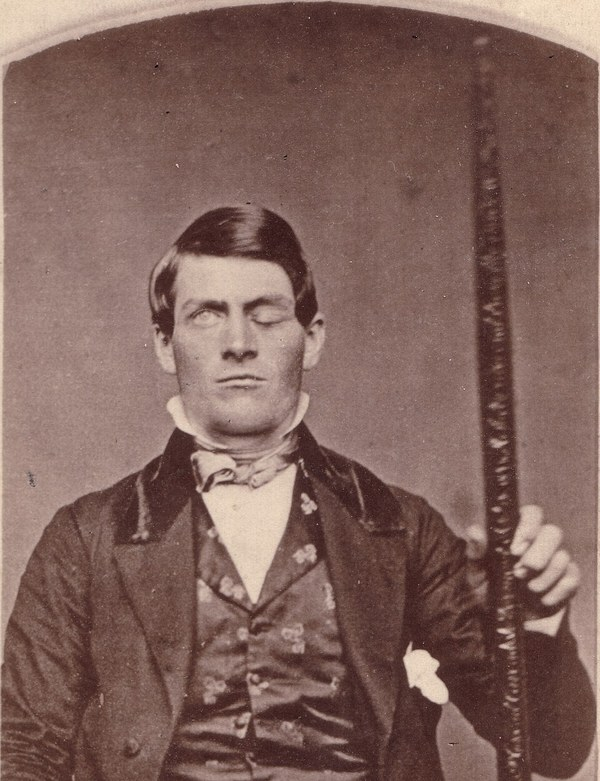
\includegraphics[height=5.0cm]{gage_portrait.jpg}\par
      {\scriptsize Գեյջը՝ իր ձողը ձեռքին}
    \end{column}
    \begin{column}{0.64\textwidth}
      \begin{itemize}
        \item Երկաթուղու շինարար, պատահական պայթյուն
        \item<2-> \textbf{Մոտ մեկ մետրանոց} երկաթյա ձողը մտավ ձախ աչքի տակից, անցավ ձախ \textbf{ճակատային բլթով} (frontal lobe) ու դուրս եկավ գանգի գագաթից
        \item<3-> Ձողն ընկավ մոտ \textbf{25 մետր} այն կողմ
      \end{itemize}
      \vspace{1mm}
      \onslide<4->{%
      \begin{bookquote}
        Մարդու գլուխը ձողին տյուլե վարագույրի չափ դիմադրություն ցույց տվեց։ Պարզաբանեմ. սա թղթով կտրվածք չէր։
      \end{bookquote}}
    \end{column}
  \end{columns}
\end{frame}

% He survived
\begin{frame}{Եվ նա ողջ մնաց}
  \begin{columns}[T]
    \begin{column}{0.5\textwidth}
      \begin{itemize}
        \item «Երկաթյա ձող գլխի միջով» այսօր էլ հարյուր տոկոսով մահացու է հնչում
        \item Իսկ սա 1800-ականներն էին, երբ ոտքի մատը խփելը կարող էր գանգրենայից մահ նշանակել
        \item<2-> Բայց Գեյջը ապրեց ևս \textbf{մոտ 12 տարի}
      \end{itemize}
      \vspace{1mm}
      \onslide<3->{%
      \begin{card}[colback=mint!35!cardwhite]
        \textbf{Ինչու}. ձողը հարթ ու սուր էր ու այնքան արագ, որ վերքը «մաքուր» ստացվեց։ Իսկ մյուս կիսագունդը ստանձնեց գործի մի մասը։
      \end{card}}
    \end{column}
    \begin{column}{0.44\textwidth}
      \onslide<4->{%
      \begin{scienceupdate}
        Գրքում՝ ձողը ոչնչացրեց ձախ ճակատային բլթի «գրեթե ամբողջը»։ 2012-ի վերակառուցումը ցույց տվեց. վնասվել էր կեղևի \textbf{մոտ 4\%}-ը, բայց սպիտակ նյութի (white matter) \textbf{10\%-ից ավելին}, այսինքն՝ մասերի միջև \textbf{կապերը}։
      \end{scienceupdate}}
    \end{column}
  \end{columns}
  \source{Van Horn et al., PLoS ONE, 2012}
\end{frame}

% The famous personality change
\begin{frame}{Նույն մարդը, թե՞ ուրիշ մարդ}
  \begin{columns}[T]
    \begin{column}{0.47\textwidth}
      \begin{card}[colback=mint!35!cardwhite]
        \centering\mascot[1.2cm]{happy}\par
        {\blackfont Մինչև վթարը}\par\smallskip
        \raggedright Մեղմ բնավորությամբ, աշխատասեր տղա
      \end{card}
    \end{column}
    \begin{column}{0.47\textwidth}
      \onslide<2->{%
      \begin{card}[colback=brainpink!30!cardwhite]
        \centering\mascot[1.2cm]{angry}\par
        {\blackfont Վթարից հետո (ըստ պատմությունների)}\par\smallskip
        \raggedright Անպատասխանատու, դյուրագրգիռ, հայհոյող, նույնիսկ «խելագար»
      \end{card}}
    \end{column}
  \end{columns}
  \vspace{1mm}
  \onslide<3->{%
  \begin{card}[colback=butter!45!cream]
    \centering Դուալիզմը լուրջ խնդրի առաջ կանգնեց. եթե ուղեղի վնասը փոխում է բնավորությունը, ուրեմն \textbf{անհատականությունն ուղեղի աշխատանքն է}։
  \end{card}}
\end{frame}

% Myth or fact: Gage never worked again
\begin{frame}{Առասպել, թե՞ փաստ \#1}
  \mythorfact{Վթարից հետո Գեյջը այլևս երբեք նորմալ չաշխատեց}{ԱՌԱՍՊԵԼ}{pinkdark}{%
    \begin{card}[colback=brainpink!25!cardwhite]
      Կյանքի վերջին տարիներին նա երկար ժամանակ \textbf{դիլիժանսի կառապան} էր. մեծ պատասխանատվությամբ ու մարդկանց հետ անընդհատ շփմամբ աշխատանք։ Եթե նույնիսկ բնավորությունը փոխվել էր, հետո նորից լավացել էր։
    \end{card}}
\end{frame}

% Why the extreme claims persist
\begin{frame}{Ինչու են պատմություններն այդքան սարսափելի}
  \begin{columns}[c]
    \begin{column}{0.56\textwidth}
      \begin{itemize}
        \item Այդ ժամանակի հոգեբանները (հարուստ, ինքնագոհ տղամարդիկ) Գեյջի դեպքով գովազդում էին \textbf{իրենց տեսությունները}
        \item<2-> Ամենածայրահեղ պնդումները հայտնվեցին \textbf{նրա մահից հետո}, երբ հերքող չկար։ Գեյջը Ֆեյսբուքից չէր իմանալու
        \item<3-> Ֆրենոլոգ Նելսոն Սայզերը գրեց, որ ձողը վնասել է «բարության» ու «ակնածանքի» «օրգանները». «դրա համար էլ հայհոյում է»
      \end{itemize}
    \end{column}
    \begin{column}{0.38\textwidth}
      \centering
      \onslide<3->{%
      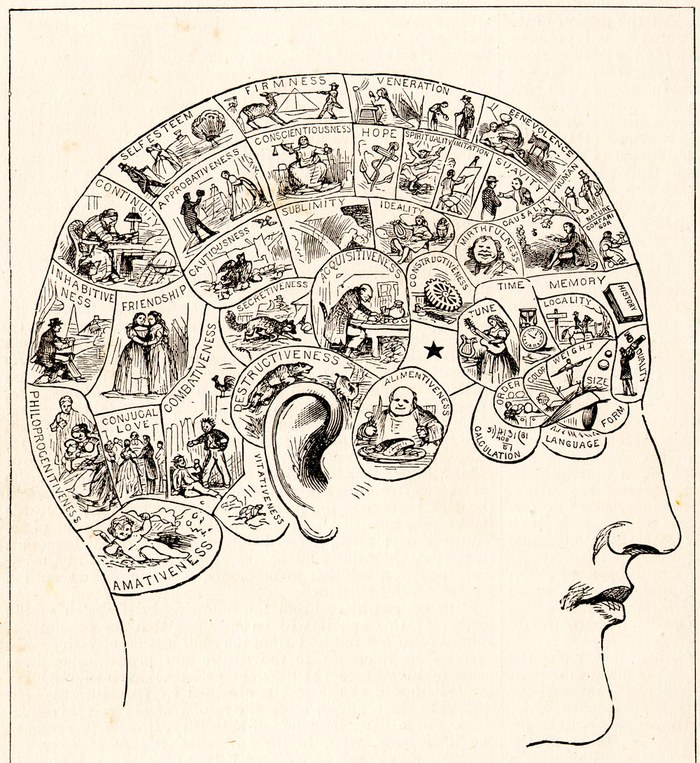
\includegraphics[height=4.8cm]{phrenology_chart.jpg}\par
      {\scriptsize Ֆրենոլոգիական քարտեզ, 19-րդ դար}}
    \end{column}
  \end{columns}
  \onslide<3->{\source{Macmillan, An Odd Kind of Fame, 2000}}
\end{frame}

% Two lasting lessons, and a definition
\begin{frame}{Գեյջի երկու դասը}
  \begin{columns}[T]
    \begin{column}{0.47\textwidth}
      \begin{card}[colback=mint!35!cardwhite]
        \emoji[1.4em]{brain}\ {\blackfont 1. Անհատականությունն ուղեղից է}\par\smallskip
        Վնասիր ուղեղը, ու մարդը կարող է փոխվել
      \end{card}
    \end{column}
    \begin{column}{0.47\textwidth}
      \onslide<2->{%
      \begin{card}[colback=peach!35!cardwhite]
        \emoji[1.4em]{ruler}\ {\blackfont 2. Այն չափելը տանջանք է}\par\smallskip
        IQ թեստերին դեռ կես դար կար։ Ինչպե՞ս չափել, թե ինչքան է Գեյջը փոխվել
      \end{card}}
    \end{column}
  \end{columns}
  \vspace{3mm}
  \onslide<3->{%
  \begin{card}[colback=lavender!35!cardwhite]
    {\blackfont\small Սահմանում, որի հետ համաձայն են հոգեբանների մեծ մասը} {\scriptsize (Phares \& Chaplin)}\par\smallskip
    Անհատականությունը մտքերի, զգացմունքների ու վարքի այն բնորոշ \textbf{նախշն} է, որը մի մարդուն \textbf{տարբերում է} մյուսից ու \textbf{պահպանվում է} ժամանակի ու իրավիճակների ընթացքում։
  \end{card}}
\end{frame}
